
%Statistics were applied to evaluate improvements in the results obtained in the performance test, user training and data clustering. A Friedmans test was used for multiple comparison and a Tukey-Kramer correction was conducted when detecting an effect. For comparison between groups in each session, a Mann-Whitney U test was applied. 
\subsubsection*{Performance Evaluation} \label{sec:R:fitts}
This section presents the results acquired from the Fitts' Law target reaching test. The test had five measures which each expresses a parameter of subjects' performance. %Subjects were divided into two groups, one test group which received exact class confidence scores during user training, and a control group which only received a single class confidence score. 
The plotted mean and standard deviations of each measure for all subjects in each group in the performance test for each session can be seen in \figref{thereIsnoFigRefYet}.
\end{multicols}

%throughput
\begin{figure}[H] 
\subfigure[]
{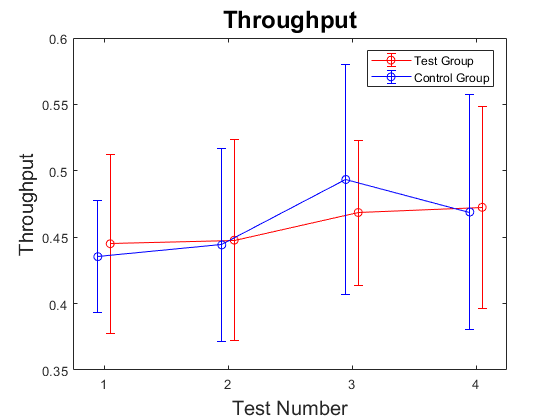
\includegraphics[width=.33\textwidth]{figures/xWesulds/Throughput}} 
\hspace{-0.5cm}
\subfigure[]
{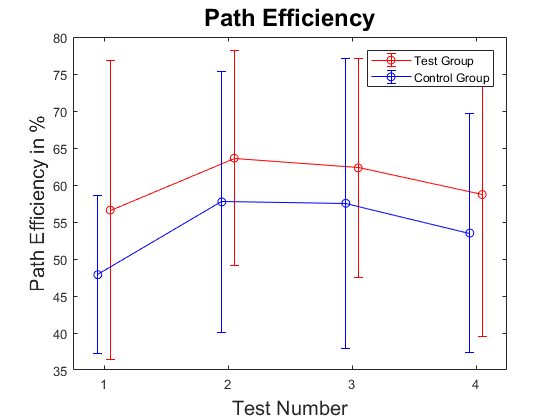
\includegraphics[width=.33\textwidth]{figures/xWesulds/PathEfficiency}} 
\hspace{-0.5cm}
\subfigure[]
{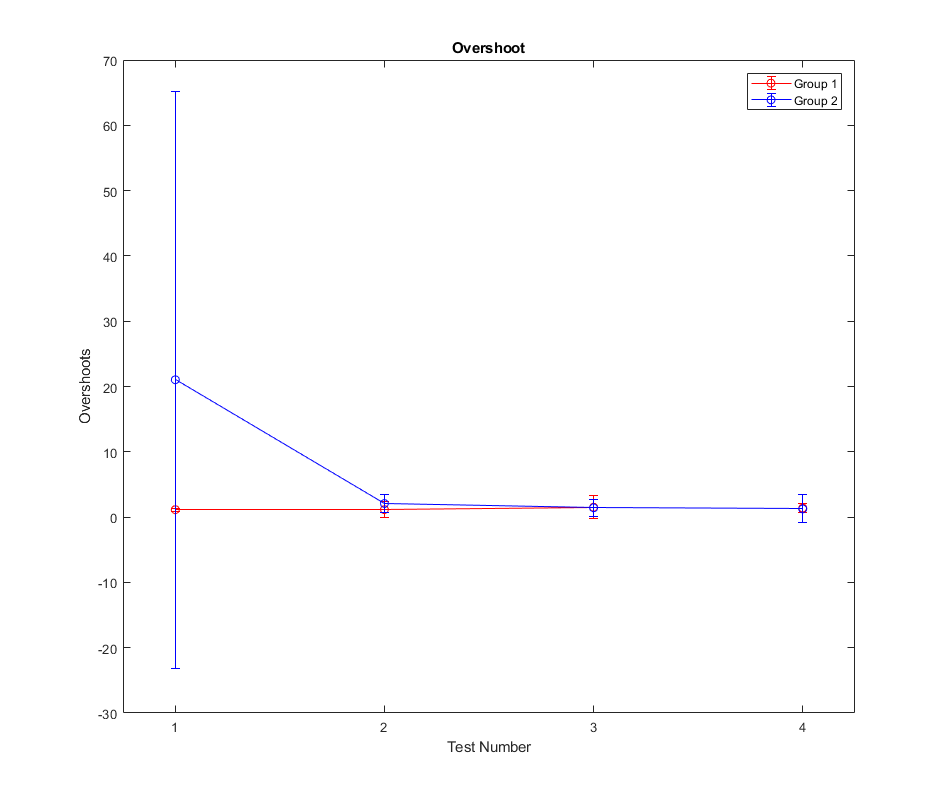
\includegraphics[width=.33\textwidth]{figures/xWesulds/Overshoot}} 
\subfigure[]
{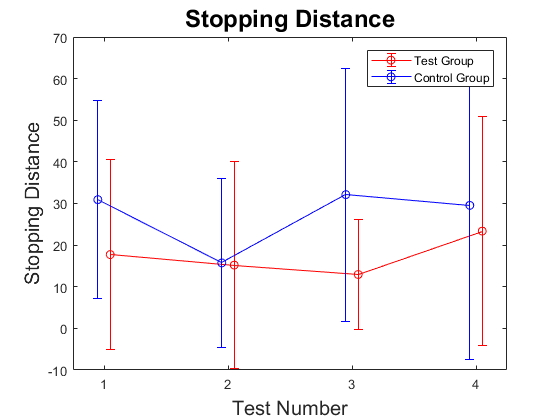
\includegraphics[width=.33\textwidth]{figures/xWesulds/StoppingDistance}} 
\hspace{-0.5cm}
\subfigure[]
{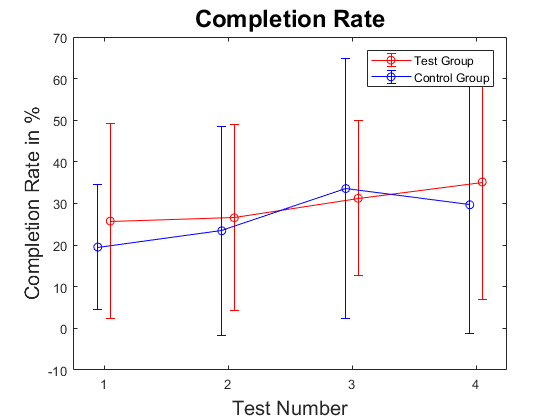
\includegraphics[width=.33\textwidth]{figures/xWesulds/CompletionRate}}  
\hspace{-0.5cm}
%\vspace{-0.5cm} 
\caption{Figure illustrating the five performance measures; \textit{ a) Throughput, b) Path efficiency, c) Overshoot, d) Stopping distance, e) Completion rate}, used for quantifying user performance across all four tests. Test number 1 is the acquired baseline used for assessing group homogeneity and the following numbers indicate performance test results after user training in each session. The red line indicates the progression of the test group and the blue line the progression of the control group.}
\label{thereIsnoFigRefYet}

\end{figure}



%
%%Path Efficiency
%\begin{figure}[H] 
%	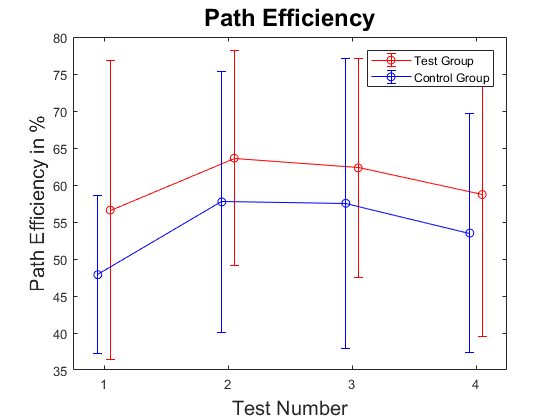
\includegraphics[width=0.3\textwidth]{figures/xWesulds/PathEfficiency}
%	\caption{Path efficiency metric for the Fitts' Law test between the test and control group.}
%	\label{fig:PEresult}
%\end{figure} 
%
%overshoot
%\begin{figure}[H] 
%	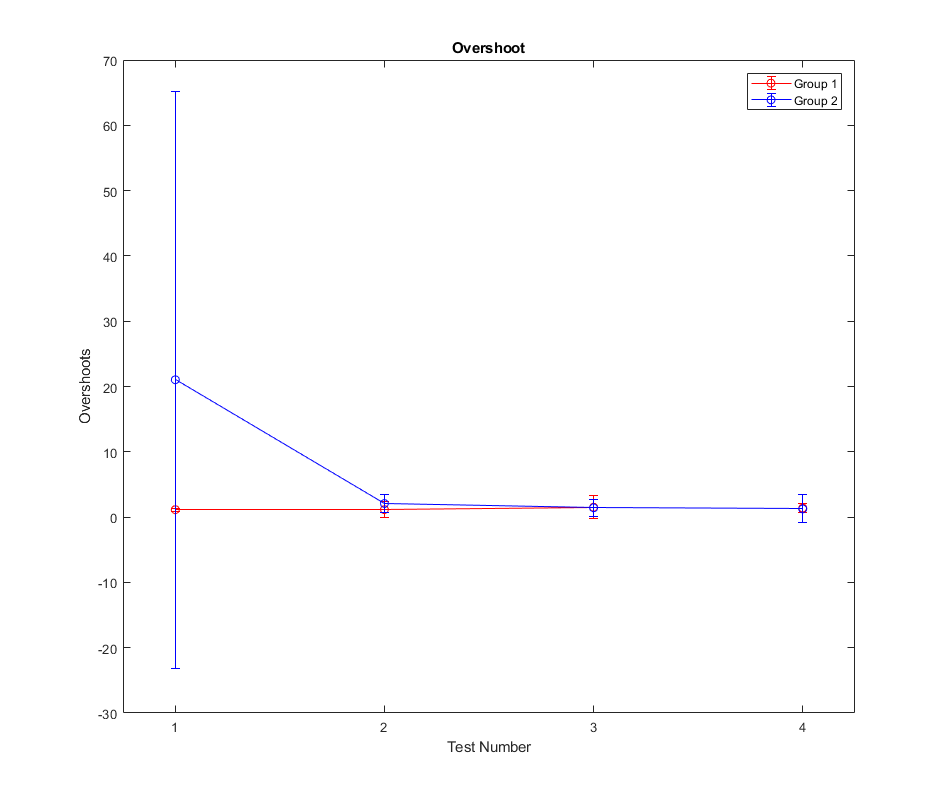
\includegraphics[width=0.3\textwidth]{figures/xWesulds/Overshoot}
%	\caption{Overshoot metric for the Fitts' Law test between the test and control group. There is no significant difference between the groups ($p > 0.05$).}
%	\label{fig:OSresult}
%\end{figure} 

%stopping distance
%\begin{figure}[H] 
%	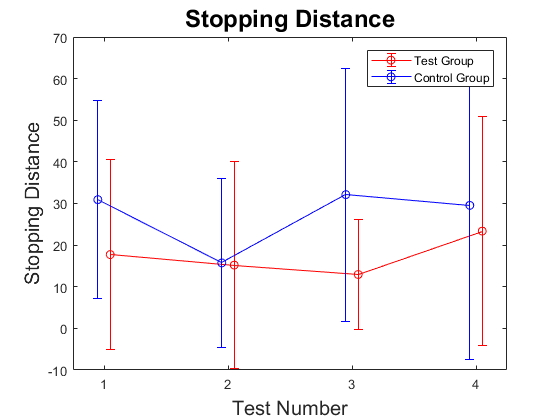
\includegraphics[width=0.3\textwidth]{figures/xWesulds/StoppingDistance}
%	\caption{Stopping distance metric for the Fitts' Law test between the test and control group. There is no significant difference between the groups ($p > 0.05$).}
%	\label{fig:SDresult}
%\end{figure} 
%
%%completion rate
%\begin{figure}[H] 
%	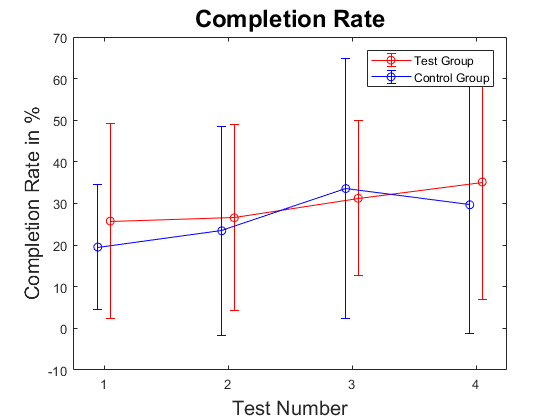
\includegraphics[width=0.3\textwidth]{figures/xWesulds/CompletionRate}
%	\caption{Completion rate metric for the Fitts' Law test between the test and control group. There is no significant difference between the groups ($p > 0.05$).}
%	\label{fig:CRresult}
%\end{figure} 
\begin{multicols}{2}
	
The baseline performance test showed no difference between the two groups, showing the two groups to be homogeneous at initiation. The Fitts' Law test results did not show any significant improvement over the three sessions for any of the five test measures for both the test and control group ($p > 0.05$). Similarly, there was no significant difference between the two groups' performance in any session ($p > 0.05$), meaning neither of them performed significantly better than the other group in any of the sessions.
\vspace{-0.5cm}




\subsubsection*{User Training Evaluation} \label{sec:R:userTraining}

This section covers the outcome measure results obtained during user training sessions. During user training subjects were instructed to train movements in being performed, such that the control system recognized the movement as the actually performed movement. \\%During this training the number of times subjects correctly performed an instructed movement to the contraction interval shown in the training interface was recorded, and will be referred to at the number of repetitions. \\
No significant difference in the total number of repetitions was found between sessions of either group ($p > 0.05$). When comparing the total number of repetitions of each session between groups accordingly, no significant difference were found either ($p > 0.05$). \\ %During user training the total completion rate is defined by the number of times a subject correctly performed a movement and held the contraction bar at the given interval for one second. A p-value of $p > 0.05$ was found for both groups in the Friedmans test comparing the performance over the three sessions, and Tukey-Kramer correction did not show any significant difference between any of the sessions ($p > 0.05$), which means there was no significant development of performance in the training for any group. 
An increased ability to get repetitions in the low intensities was found for the control group ($p < 0.05$, session 1 $ = 16.13 \pm 5.59$, session 3 $= 21.38 \pm 6.78$). Otherwise, no significant difference were yielded for both groups when comparing the subjects' ability to reach the three other contraction levels between sessions ($p > 0.05$).
%Friedmans test was applied to examine if there was a development in the ability to reach the different contraction levels within the three training sessions. A p-value of $p > 0.05$ was found for both groups, with the Tukey-Kramer correction yielding $p > 0.05$ for the comparison of the three sessions, meaning there was no change in ability to reach different intensities.
No difference was found, when comparing the two groups' ability to reach different intensities during training either ($p > 0.05$). \\
Comparing the ability to perform different movements during the training showed a significant improvement for the test group in ulnar deviation ($p < 0.05$, session 1 $ = 11.38 \pm 4.27$, session 3 $= 16.13 \pm 2.95$) and open hand ($p < 0.05$, session 1 $ = 11.25 \pm 3.85$, session 3 $ = 17.88 \pm 2.46$). A significant decrease in performance was found for the control group's ability to perform flexion ($p < 0.05$, session 2 $ = 16.63 \pm 2.77$, session 3 $ = 11.00 \pm 3.16$). Otherwise, no significant difference between the three sessions for the two groups was found ($p > 0.05$).\\ %, with the Tukey-Kramer correction resulting in $p > 0.05$ between all sessions for both the test and control group, meaning there was no development in ability to reach specific positions. 
A significant difference ($p < 0.05$) was found between the test and control group's ability to reach the closed hand movement, with a mean of $26.8 \pm13.5$ number of repetitions for the test group and $38 \pm12.2$ for the control group. No significant difference was found for any of the other movements when comparing the two groups ($p > 0.05$).

\subsubsection*{Cluster Dispersion and Separability}
In this section, results from the data acquisition are presented. The data used for training the LDA based classifier was examined. Each movement resulted in a cluster of data points, which was examined in order to analyse the change in cluster dispersion and distance between cluster centroids. \\
For both groups the mean distance between the cluster centroids were calculated. The change in between cluster distances over the three sessions were tested and showed no significant difference ($p > 0.05$). Likewise, no significant difference in the development of cluster distances between the groups was found ($p > 0.05$).\\
The mean distance from data points to the cluster centroid was calculated. This showed no significant difference for the test group ($p > 0.05$), but a significant difference was found for the control group ($p < 0.05$). The Tukey-Kramer correction showed the significant difference was between session one and three ($p < 0.05$), where the mean for session one was $502.02 \pm 274.88$ arb. unit, and session three was $323.43 \pm 171.13$ arb. unit. The comparison between groups showed that the control group achieved a significant improvement in cluster dispersion compared to the test group in session three ($p < 0.05$), where the test group had a mean cluster dispersion of $584.34 \pm 250.02$ arb. unit, while the control group had $323.43 \pm 171.13$ arb. unit. 
%\end{multicols}